% This is samplepaper.tex, a sample chapter demonstrating the
% LLNCS macro package for Springer Computer Science proceedings;
% Version 2.20 of 2017/10/04
%
\documentclass{llncs}
\pagestyle{plain}
\bibliographystyle{splncs04}
\setcounter{tocdepth}{2}
\makeatletter
\renewcommand*\l@author[2]{}
\renewcommand*\l@title[2]{}
\makeatletter
\usepackage[bookmarks]{hyperref}
%
\usepackage{graphicx}
\usepackage{minted}
\usepackage{longtable}
% If you use the hyperref package, please uncomment the following line
% to display URLs in blue roman font according to Springer's eBook style:
\renewcommand\UrlFont{\color{blue}\rmfamily}
\newcommand{\hs}{\mintinline{haskell}}
\usepackage{todonotes}

\begin{document}
%
\title{Concurrency Oracles for Free}

%\titlerunning{Abbreviated paper title}
% If the paper title is too long for the running head, you can set
% an abbreviated paper title here
%
\author{Georgy Lukyanov \and Andrey Mokhov}
%
% \authorrunning{F. Author et al.}
% First names are abbreviated in the running head.
% If there are more than two authors, 'et al.' is used.
%
\institute{School of Engineering, Newcastle University, United Kingdom}

\maketitle

\begin{abstract}
This paper presents an approach to deriving \emph{concurrency oracles} for
processor instructions whose behaviour is formally specified using a state
transformer semantics. The presented approach does not require any modification
of the existing semantics, nor does it rely on writing a parser for the language
in which the semantics is described, thus justifying the ``for free'' part of
the title.

The main tool in our arsenal is \emph{ad-hoc polymorphism}: the presented
approach is only applicable when the semantics of processor instructions is
expressed using state transformation functions that can be reinterpreted in
different contexts. As we show in the paper, such semantics can be interpreted
not only for instruction simulation or verification, but also for extracting the
information about instruction dependencies, thus allowing us to identify
concurrency as well as various types of conflicts between instructions or blocks
of instructions.

\keywords{concurrency oracle
\and instruction set architecture
\and functional programming
\and polymorphism}
\end{abstract}
% \tableofcontents

\section{Introduction and motivation\label{sec:intro}}
Deciding whether two given events in a trace are \emph{concurrent}, i.e. have
no causal or data dependencies between them, is a major problem in the process
discovery field~\cite{2011_aalst_book}. Various methods for concurrency
extraction, often referred to as \emph{concurrency oracles}, have been
introduced, including the classic $\alpha$-algorithm~\cite{van2004workflow}, as
well as a few less widely known methods, e.g. see~\cite{cook1998event},
\cite{mokhov2016mining} and the review paper~\cite{augusto2017automated}. A
good example of treating a concurrency oracle as a self-contained problem can
be found in~\cite{dumas2015process}.

In this paper we present an approach for deriving concurrency oracles for
events that correspond to processor instructions and blocks of instructions. The
input to the proposed approach is the \emph{microarchitectural semantics} of
instructions, which gives a precise description of how an instruction execution
changes the state of the processor.

A popular method to describe microarchitectural semantics is to use a dedicated
domain-specific language embedded in a high-level general-purpose host language,
such as Haskell or Coq. Two pioneering works in this domain
are~\cite{fox2010trustworthy}, where the Arm v7 instruction set architecture
is formalised in HOL4, and~\cite{kennedy2013coq}, where x86 architecture is
formalised in Coq.

The authors of this paper have also used an embedded domain-specific language
to describe the semantics of a space-grade
microarchitecture~\cite{mokhov2018formal}. In particular, it was demonstrated
that the same semantics can be reused in different contexts: to simulate the
processor and to perform formal verification of programs executed by the
processor. In this paper we take this work further, by demonstrating that the
very same semantics can be reused for deriving concurrency oracles that given
two instructions, or blocks of instructions, can determine whether they are
concurrent and, if not, report the data dependency conflicts.

We start by studying several common examples of processor instructions, noticing
that different instructions require different features from the language used to
describe them; see~\S\ref{sec:instructions}. We proceed by introducing the
language for specifying semantics in more detail and then describe the semantics
of a small instruction set (\S\ref{sec:metalanguage}). The approach to deriving
concurrency oracles is presented in~\S\ref{sec:oracles}, followed by a
discussion.


\vspace{-1mm}
\section{Instruction set architecture semantics\label{sec:instructions}}
\vspace{-2mm}
In this section we introduce the computational metalanguage by example. We will
use the metalanguage to describe the semantics of a part of a simple generic instruction
set architecture. The later sections will introduce a formal definition of the
metalanguage, instruction and program semantics and present a method of extracting static
data dependencies of instructions with certain properties from the semantic definitions
leading to a construction of a~\emph{concurrent oracle}.

\begin{figure}[H]
\includegraphics[width=35em]{img/loadJumpAdd.pdf}
\caption{Static data dependencies of~\hs{Load R0 0},~\hs{Add R1 1} and~\hs{Jump 42} instructions.}
\end{figure}

\subsubsection{Unconstrained semantics. Load} Literally every real-world instruction set include an instruction
which loads a data word from a memory location to a register. Here is how the
semantics of such an instruction can be encoded in the metalanguage:

\begin{minted}{haskell}
load reg addr = \read write -> Just $
    write (Reg reg) (read (Addr addr))
\end{minted}

In this definition we use two metalanguage terms:~\hs{read} and~\hs{write} to encode
the behaviour. These terms are polymorphic effectful functions with the following
types:

\begin{minted}{haskell}
read :: MachineKey -> f Word64
read =

write :: MachineKey -> f Word64 -> f ()
write =
\end{minted}

The~\hs{read} term queries the microarchitectural state for the value of a key and
returns it wrapped in a context~\hs{f}, which is, in fact, the reason for the
metalanguage to be~\emph{polymorphic}. In this case the context~\hs{f} may be any
type constructor of kind~\hs{* -> *}. However, not every instruction semantics may
be expressed in an unconstrained context. Let us consider semantics of some other
instructions to elaborate more on the nature of~\hs{f}.

\subsubsection{Functorial semantics. Jump}

Another popular instruction is the unconditional control flow transfer:

\begin{minted}{haskell}
jump offset = \read write -> Just $
    write IC ((+ offset) <$> (read IC))
\end{minted}

The semantics of this instruction increments the instruction counter~\hs{IC}
to transfer the control to another instruction in the program. This definition
has an crucial difference from~\hs{load}: it uses
the~\hs{<$>}\footnote{Function~\hs{<$>} (pronounced "fmap") of type
\hs{Functor f => (a -> b) -> f a -> f b} allows to transform the values in an
computational context with a pure function.} function of the~\hs{Functor} type
class, thus restricting~\hs{f} to be a~\hs{Functor}:

\begin{minted}{haskell}
read :: Functor f => MachineKey -> f Word64
read =

write :: Functor f => MachineKey -> f Word64 -> f ()
write =
\end{minted}

In this definition functorial constraint is required to apply the increment function
~\hs{(+ offset) :: Num a => a -> a} to the instruction counter enclosed in a computational
context~\hs{f}.

Later in the paper we will instantiate~\hs{f} as a context of data dependency
tracking. It turns out that the~\hs{Functor} constraint is equivalent to stating
that a computation may have at most one static dependency, being the instruction
counter in the case of~\hs{load}.

\subsubsection{Applicative semantics. Add}

The~\hs{add} instruction semantics performs the addition of the values of
a register and a memory cell. If the result of the addition is equal to zero,
the semantics sets the~\hs{Zero} microarchitectural flag~\hs{True}, or to~\hs{False} otherwise.

The Haskell definition of the semantic function is a bit more involved than the previous
ones. It turns out that the~\hs{Functor} context is not expressive enough and a
more powerful abstraction is needed. The following definition of~\hs{add} requires
\hs{f} to be at least an~\hs{Applicative}:

\begin{minted}{haskell}
add reg addr = \read write -> Just $
    let result = (+)    <$> read (Reg reg) <*> read (Addr addr)
        isZero = (== 0) <$> result
    in  write (Reg reg) result *>
        write (F Zero)  isZero
\end{minted}

Let us describe what is going on here. The definition may be broken down in three
classes of actions: reading data, processing it on-the-fly and writing data back in the store.

The first~\hs{let}-binding uses~\hs{Applicative} notation
to read the values from the register and memory address and add them up. Note that
this notation is~\emph{declarative}, hence it rather states that the~\hs{result}
is supposed to be a sum of values of two entities than performs actual computation.
This intuition is very important for understanding the static dependency tracking semantics
of instructions:~\hs{Reg reg} and~\hs{Addr addr} are declared as static input dependencies of
the~\hs{add} instruction. However, since the semantics may be executed in any~\hs{Applicative} context,
this dependency-tracking inspired intuition must not
obscure other possible interpretations of the semantics. For instance, in a stateful
simulation context, the~\hs{result} will be computed based on concrete data values
read from the underlying store.

The second line of the~\hs{let}-binding is quite similar to the expression in the
semantics of the~\hs{jump} instruction. The type of the~\hs{result} is~\hs{f Word64},
hence the zero testing function~\hs{(==) 0} of type~\hs{(Num a, Eq a) => a -> Bool}
must be mapped over the context~\hs{f} with~\hs{<$>} to obtain the value of type
\hs{f Bool}.

The latter two lines of the definition perform two~\hs{write} operations chained with
the applicative notation combinator~\hs{*>} of type~\hs{Applicative f => f a -> f b -> f b}.
This declares the values~\hs{Reg reg} and~\hs{F Zero} to be output dependencies of
the computation and that the writes mush be both performed.

An interesting feature of the~\hs{Applicative} notation is that it does not specify the exact order of
performing actions. This feature is useful in embedded domain-specific languages
with concurrency, for instance Facebook's Haxl~\cite{Marlow:2014:NFA:2692915.2628144}.

\hs{Applicative} functors are powerful enough to express the semantics of a
large class of instructions. In this paper we exploit their features to not only
specify the execution semantics but also automatically track static data dependencies
of instructions. However not every instruction of modern architecture may be
equipped with~\hs{Applicative} semantics. If the behaviour start to depend on the
actual data, i.e.~\emph{dynamic} data dependencies emerge, the semantics can not
be encoded using an~\hs{Applicative}. A more powerful abstraction is required.

\subsubsection{Monadic semantics. Memory indirect Load}

The indirect memory access instruction looks up a value in a memory cell and uses
it as the effective address in the regular load instruction. Since the effective
address can not be determined statically in the general case, this instruction
has a dynamic data dependency. The polymorphic computational metalanguage requires
the context~\hs{f} to be a~\hs{Monad} in order to be able to encode such behaviour.
Consider the definition of the semantics of the~\hs{loadMI} instruction, which
uses Haskell monadic ~\hs{do}-notation:

\begin{minted}{haskell}
loadMI reg addr read write = Just $ do
    addr' <- read (Addr addr)
    write (Reg reg) (read (Addr addr'))
\end{minted}

The first line extracts the effective address from the monadic context
and binds the identifier~\hs{addr'} to it. Here is the catch: expressions
on left-hand-side and right-hand-side of the~\hs{<-} symbol have different types.
The~\hs{read (Addr addr)} is of type~\hs{Monad f => f MemoryAddress} and the
identifier~\hs{addr'} has type \hs{MemoryAddress}. The main feature of~\hs{Monad}
is ability to extract a value from an effectful context and pass it in the further
computation as it was pure. This gives us a possibility to pass the~\hs{addr'}
as an argument to the next~\hs{read} operation.

Monadic semantics is more powerful that unconstrained, functorial and applicative ones,
but we are no more able to extract all the dependencies of the computation if
\hs{f} is restricted to~\hs{Monad}, since some of them will not be static. Therefore,
concurrency oracles can not be built for~\hs{Monad}-flavoured computations.

We have given examples of four kinds of semantic computations: unrestricted, functorial,
applicative and monadic. In every definition we used functions~\hs{read} and~\hs{write}
and have constrained the context~\hs{f} with~\hs{Functor},~\hs{Applicative}
or~\hs{Monad}. The resulting types of~\hs{read} and~\hs{write} follow a certain
pattern, which may be encoded in the Haskell type system. In fact, a generic
~\hs{read} may be assigned with type~\hs{forall c. MachineKey -> (c f) Word64} and
generic~\hs{write} with~\hs{forall c. MachineKey -> (c f) Word64 -> (c f) ()}. Here,
type variable~\hs{c} mush have kind~\hs{* -> Constraint}. This allows to instantiate
~\hs{c} with~\hs{Functor}, \hs{Applicative}, \hs{Monad} or any other suitable constraint,
thus making the metalanguage polymorphic in the computational context.

The next section will present a formal definition of the metalanguage, instruction
and program semantics. The section~\ref{oracles} will describe the construction of
concurrency oracles for programs comprising unrestricted, functorial, applicative,
but not monadic instructions.



\section{Polymorphic computational metalanguage\label{sec:metalanguage}}
This section present a framework for describing the semantics of programming languages
in terms of a~\emph{polymorphic computational metalanguage}. We call the metalanguage
polymorphic because, once semantics is encoded in the metalanguage,
it may be evaluated in different contexts yielding meanings of a computation
flavoured by the context.

\begin{definition}
\label{def:metalanguage}
\textbf{Polymorphic computational metalanguage}\\
A polymorphic computational metalanguage is a type constructor $F$ equipped with
two effectful functions: $\forall k \forall v.r: k \rightarrow F v$ and
$\forall k \forall v.w: k \rightarrow F v \rightarrow F~\top$.
\end{definition}

We embed the metalanguage in Haskell using the following type:

\begin{minted}{haskell}
type Semantics c k v a = forall f. c f => (k -> f v)
                                       -> (k -> f v -> f ())
                                       -> Maybe (f a)
\end{minted}

A~\hs{Semantics} is essentially a rank-2 polymorphic\footnote{A rank-2 polymorphic
function is one taking as a parameter another function, which is in turn (rank-1)
polymorphic. This feature requires~\hs{RankNTypes} GHC extension to be enabled.}
effectful computation depending on two polymorphic functions,
which we will usually referred to as~\hs{read} and~\hs{write}.

Let us now give some intuition for the components of the metalanguage.
The~\hs{Semantics c k v a}
type may be thought as a mutable dictionary. The types~\hs{k} and~\hs{v} represent keys
and associated values. The~\hs{read} function has type~\hs{k -> f v} --- it takes
a key and gives back an effectful value looked up in the dictionary. The~\hs{write}
function takes a key and an effectful value to and alters the value of the key
with the value. The semantics is allowed to fail to produce a result, hence the
the return type~hs{f a} is wrapped in the~\hs{Maybe} type constructor.~\hs{Maybe}
\footnote{This type is defined in the Haskell base library as~\hs{data Maybe a = Just a | Nothing}}
is an idiomatic Haskell encoding of potentially faulty computations.

In this paper we use the defined metalanguage to encode the semantics of the
instruction set architecture of a simple computer. We call this computer
IAM~\footnote{Inglorious Haskell Machine}. The next section gives an overview of
its microarchitecture and instruction set, present the semantics of instructions
and programs in terms of the polymorphic computational metalanguage and two
instantiations of the semantics: stateful simulator and concurrent data access
analyser.



% Let us give an intuition on the possible evaluation contexts.
% Probably the most obvious one for an is stateful execution;
% interpreting the semantics in the~\hs{State} monad will yield
% a simulator giving users the possibility to execute computations and observe
% their behaviours.

% Another interesting task is to build a~\emph{concurrency oracle} for computations.
% A concurrency oracle is a function, which is able to identify if two computations
% are~\emph{concurrent}, i.e. do not share any data dependencies.
% In the section section~\ref{sec:oracles} we present a method of extracting
% such oracles from the semantic definitions with certain properties.





\section{Concurrency oracles\label{sec:oracles}}
In this section we present a method to derive concurrency oracles from the instruction
semantics encoded in the  metalanguage (Definition~\ref{def:metalanguage}).
More specifically, we aim to reason about instructions that
have only \emph{static dependencies}.

We start by introducing formal definitions and Haskell encodings of the concepts
required for building concurrency oracles.
First, we define the notions of input and output dependencies of a computation.

\textbf{Definition (input dependency):\label{def:in-dependencies}}
Consider a term $f$ of an applicative metalanguage~\hs{Semantics Applicative a}.
A key $k$ is an~\emph{input dependency} of the term $f$ if the term $f$
performs a~\hs{read} of the key $k$.

\textbf{Definition (output dependency):\label{def:out-dependencies}}
Consider a term $f$ of an applicative metalanguage~\hs{Semantics Applicative a}.
A key $k$ is an~\emph{output dependency} of the term $f$ if the term $f$
performs a~\hs{write} of the key $k$.

\textbf{Definition (dependencies):\label{def:dependencies}}
Consider a term $f$ of an applicative metalanguage~\hs{Semantics Applicative a}.
The~\emph{dependencies} of the term $f$ are sets $I$ and $O$ -- the input and
output dependencies of the term $f$, respectively.

In the Haskell implementation, we do not distinguish between input and output dependencies
in the type level, thus the function determining the dependencies of a computation
has the following type:

\begin{minted}[xleftmargin=10pt]{haskell}
dependencies :: Semantics Applicative a -> Maybe ([Key], [Key])
\end{minted}

\noindent
The~\hs{Maybe} type constructor comes from the definition of the metalanguage:
if the applicative semantics is partial (returns~\hs{Nothing}) it is impossible
to extract its static dependencies. Successful static analysis yields a pair of
lists representing the sets of input and output dependencies of a computation.

To extract the static data dependencies of an applicative computation we need to
interpret its semantics in the special context of a \emph{constant functor}.

\subsection{The constant functor}

The~\hs{Const a b} data type is defined as follows~\cite{Mcbride:2008:APE:1348940.1348941}:

\begin{minted}[xleftmargin=10pt]{haskell}
newtype Const a b = Const { getConst :: a }
\end{minted}

\noindent
A value of the~\hs{Const a b} is just a value of any type~\hs{a}
wrapped in a data constructor. However, it is important that the type constructor
has a~\emph{phantom type} variable. This type variable allows us to
declare useful instances of standard Haskell type classes such as~\hs{Functor}
and \hs{Applicative} for \hs{Const a}. We would like to use this data type as a
computational context for applicative semantics, hence we declare the
corresponding instance\footnote{\hs{Const a} also has a \hs{Functor} instance,
where~\hs{fmap _ (Const x) = Const x}.}:

\begin{minted}[xleftmargin=10pt]{haskell}
instance Monoid m => Applicative (Const m) where
    pure _              = Const mempty
    Const x <*> Const y = Const (x `mappend` y)
\end{minted}

This instance exactly describes the desired behaviour of static dependency tracking
computational context.~\hs{Const [Key]} is an applicative functor that ignores
its enclosed value, but accumulates the declared dependencies using the~\hs{Monoid}
instance for Haskell list data type\footnote{The empty list~\hs{[]} is the
monoid identity element and the list concatenation~\hs{(++)} is the associative
binary operation.}.

\subsection{Extracting dependencies}

Using the seemingly vacuous datatype \hs{Const} we define the
function \hs{dependencies}:

\begin{minted}[xleftmargin=10pt]{haskell}
dependencies :: Semantics Applicative a -> Maybe ([Key], [Key])
dependencies s = partitionEithers . getConst <$> s read write
  where read  k    =       Const [Left  k]
        write k fv = fv *> Const [Right k]
\end{minted}

\noindent
We instantiate the polymorphic computation context with \hs{f = Const [Key]}
and supply custom tracking \hs{read} and \hs{write} functions. In fact, \hs{read}
does not perform any reading and just tracks the key as an input dependency,
whereas \hs{write} tracks the key as an output dependency and executes the
effectful computation \hs{fv}, to appropriately track its dependencies. The
resulting list of keys gets unwrapped and unzipped by standard
\hs{partitionEithers}~\hs{.}~\hs{getConst}.

This whole paper is built around the above three-line implementation of the
function \hs{dependencies}: the rest is just functional programming background
and folklore, which is required for understanding these three lines of code.

Fully armed with static dependency analysis, we can now define concurrency
oracles for programs written in the presented metalanguage.

\subsection{Concurrency oracle}
% \vspace{-2em}
A concurrency oracle is a function taking two computations and statically
determining if they are data~\emph{concurrent}, i.e. do not share any
data dependencies.


\textbf{Definition (Concurrency Oracle Answer):\label{def:concurrency-status}}
Two terms of the metalanguage are \emph{concurrent} if they do not share any
data dependencies. They are in a \emph{read} or \emph{write conflict} if they
share any input or output dependencies, respectively. If the share both input
and output dependencies then they are considered to be in a \emph{read-write
conflict}. We use the following data type is used to encode concurrency oracle
answers:

\begin{minted}[xleftmargin=10pt]{haskell}
data OracleAnswer k = Concurrent
                    | ReadConflict [k]
                    | WriteConflict [k]
                    | ReadWriteConflict [k]
\end{minted}

\textbf{Definition (concurrency oracle):\label{def:oracle}}
Consider two terms with applicative semantics \hs{s1} and \hs{s2} of the
type~\hs{Semantics Applicative a}. A~\emph{concurrency oracle} is a
function of the following type:
% \vspace{-3em}
\begin{minted}[xleftmargin=10pt]{haskell}
concurrencyOracle :: Eq k => Semantics Applicative k v1 a
                          -> Semantics Applicative k v2 a
                          -> Maybe (OracleAnswer k)
\end{minted}

\noindent
The function is required to return \hs{Nothing} when one of the given semantics
is undefined, e.g. if it corresponds to an instruction with dynamic dependencies.
Below is one possible implementation:

\begin{minted}[xleftmargin=10pt]{haskell}
concurrencyOracle s1 s2 = do
    (r1, w1) <- dependencies s1
    (r2, w2) <- dependencies s2
    let readConflicts      = intersect r1 r2
        writeConflicts     = intersect w1 w2
        readWriteConflicts = intersect (r1 ++ w1) (r2 ++ w2)
    pure $ case (readConflicts, writeConflicts, readWriteConflicts) of
        ([], [], [] ) -> Concurrent
        (rs, [], rws) | rs == rws -> ReadConflict rs
        ([], ws, rws) | ws == rws -> WriteConflict ws
        (_ , _ , rws) -> ReadWriteConflict rws
\end{minted}
% \vspace{-3em}

The oracle determines static dependencies of two given terms and examines
several possible cases of the intersections of their input and output
dependencies.

\subsection{Example oracles}

In this subsection we show two examples to illustrate the usage of concurrency
oracles. The examples are given in the form of interactive sessions, where
`\hs{ghci>}' denotes the command prompt.

Two \hs{Load} instructions with different arguments are concurrent as confirmed
by the oracle returning the result \hs{Just Concurrent}:

\begin{minted}[xleftmargin=10pt]{haskell}
ghci> concurrencyOracle (semanticsA (Load R0 0))
                        (semanticsA (Load R1 1))
Just Concurrent
\end{minted}

\noindent
Extending the first computation with an additional \hs{Add} instruction causes
a read conflict, as desired:
\begin{minted}[xleftmargin=10pt]{haskell}
ghci> p1 = blockSemanticsA [Load R0 0, Add R0 1]
ghci> p2 = semanticsA (Load R1 1)
ghci> concurrencyOracle p1 p2
Just (ReadConflict [Addr 1])
\end{minted}

\noindent
We can overlay dependency graphs of programs \hs{p1} and \hs{p2} as follows (we
place the programs at starting addresses 10 and 20, respectively):

\begin{minted}[xleftmargin=10pt]{haskell}
ghci> Just g1 = programDataGraph (zip [10..] [Load R0 0, Add R0 1])
ghci> Just g2 = programDataGraph (zip [20..] [Load R1 1])
ghci> drawGraph (overlay g1 g2)
\end{minted}

\noindent
The resulting dependency graph is shown in Fig.~\ref{fig-example-graph}.
% In the graph, instructions labelled with 1 and 2 belong to the blocks~\hs{p1}
% and~\hs{p2} respectively.
As one can see, the programs have a read conflict on key \hs{Addr 1},
just like the oracle has determined.

\begin{figure}
\vspace{-4mm}
\centerline{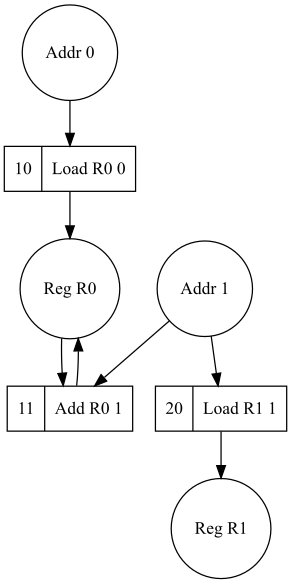
\includegraphics[scale=0.6]{img/oracle2.pdf}}
\vspace{-3mm}
\caption{An overlay of static dependency graphs of two blocks of instructions.\label{fig-example-graph}}
\vspace{-9mm}
\end{figure}


\section{Synthesis of efficient hardware microcontrollers\label{sec:scenarios}}
In this section, we present a method for extracting behavioural~\emph{scenarios} from
system control programs and synthesising them into application-specific
integrated circuits implementing execution of these scenarios. We exploit the
existing formalism of Conditional Partial Order Graphs (CPOGs)~\cite{cpogs} for
synthesising scenarios. CPOGs are included~\cite{scenco} as a plugin in the WORKCRAFT
framework~\cite{workcraft}, which implements the scenario specification and
synthesis methods and handles the mapping of CPOGs into interconnection of
logic gates to produce a physical implementation of the system microcontroller.

\subsection{Extracting scenarios from programs}

We defined a \textit{scenario} to be a list of
operations that are executed in a specified order. Formally, a scenario
$s=(\mathcal{O},\prec)$ is a \textit{partial order}~(PO)~\cite{PO},
i.e. a binary precedence relation $\prec$ describing dependencies between a
set of operations $\mathcal{O}$ that satisfies two properties:

\begin{itemize}
    \item Irreflexivity: $\forall a \in \mathcal{O}, \neg(a \prec a)$
    \vspace{+1mm}
    \item Transitivity: $\forall a, b, c \in \mathcal{O}, (a \prec b) \wedge (b
    \prec c) \Rightarrow (a \prec c)$
\end{itemize}

To mine scenarios from blocks of instructions, we partially reuse the methodology
used for construction of the concurrency oracles from the previous section.

The methodology is realised as the following informal algorithm:

\begin{enumerate}
    \item Calculating the static data dependencies of the program.
    \item Construct the~\emph{unfolded} static dependencies
        graph~\footnote{Similar to one in the figure~\ref{fig-example-graph},
        but with with data-vertexes duplicated on every update.}
    \item Remove the data-vertexes preserving the transitive connections between
        instruction-vertexes.
    \item A~\emph{transitive closure} of the resulting graph will display the
        partial order on the set of events represented as instruction-vertexes.
\end{enumerate}

As an example, consider a program for the control unit of a hypothetical dual-motor
autonomous vehicle. The motor's velocity may be adjusted with the command~\hs{AdjustVelocity}
supplying the value in a register and referring the motor index (0 or 1). The status
of the system may be checked with the~\hs{SystemStatus} command, referring both motors
and a register to store the resulting status code.

\begin{figure}
\vspace{-10mm}
\centering
  \begin{minipage}[b]{0.5\textwidth}
\begin{minted}[linenos]{haskell}
Load R0 254
AdjustVelocity R0 0
AdjustVelocity R0 1
SystemStatus R2 0 1
\end{minted}
\vspace{5mm}
\end{minipage}
% \hfill
\begin{minipage}[b]{0.4\textwidth}
\includegraphics[scale=0.35]{img/ataed-scenario-1.pdf}
\end{minipage}
\caption{Simple behaviour scenario and the corresponding partial order.}
\end{figure}

Extraction of scenarios from programs enables us to use the associated methods for
compiling programs into application-specific hardware. The Conditional Partial
Order Graphs formalism enables synthesis of scenarios, allowing to compile them into
a circuit with some functionality shared.

Consider the above mentioned scenario synthesised with another one into a single
partial order which shares similar functionality.

\begin{figure}
\vspace{-4mm}
\centerline{\includegraphics[scale=0.4]{img/ataed-composition.pdf}}
\caption{Two operation scenarios and their composition.\label{fig-scenarios}}
\vspace{-9mm}
\end{figure}

asdasdasdasdasdasd

\section{Conclusion}
The paper presents a polymorphic metalanguage for describing semantics of
instruction set architecture. The metalanguage closely resembles state transformers.
The polymorphism of the metalanguage combinators allows to evaluate the semantics
of instruction in different contexts without anyhow modifying the semantics itself.
As the primary application, we present an approach to deriving concurrency oracles
of the instructions with only static data dependencies.
%
% ---- Bibliography ----
%
% BibTeX users should specify bibliography style 'splncs04'.
% References will then be sorted and formatted in the correct style.
%
\bibliography{biblio}
\end{document}
